\documentclass{article}

\usepackage{amsmath}
\usepackage{amsthm}
\usepackage{amssymb}
\usepackage{bm}
\usepackage{bbm}
\usepackage{fancyhdr}
% \usepackage{listings}
\usepackage{cite}
\usepackage{graphicx}
\usepackage{enumitem}
\usepackage{courier}
\usepackage[pdftex,colorlinks=true, urlcolor = blue]{hyperref}
\usepackage{pdfpages}

% Preamble for tikz generated via mathcha.io
\usepackage{physics}
\usepackage{amsmath}
\usepackage{tikz}
\usepackage{mathdots}
\usepackage{yhmath}
\usepackage{cancel}
\usepackage{color}
\usepackage{siunitx}
\usepackage{array}
\usepackage{multirow}
\usepackage{amssymb}
\usepackage{gensymb}
\usepackage{tabularx}
\usepackage{booktabs}
\usetikzlibrary{fadings}
\usetikzlibrary{patterns}
\usetikzlibrary{shadows.blur}
\usetikzlibrary{shapes}


\oddsidemargin 0in \evensidemargin 0in
\topmargin -0.5in \headheight 0.25in \headsep 0.25in
\textwidth 6.5in \textheight 9in
\parskip 6pt \parindent 0in \footskip 20pt

% set the header up
\fancyhead{}
\fancyhead[L]{Stanford Aeronautics \& Astronautics}
\fancyhead[R]{Fall 2020}

%%%%%%%%%%%%%%%%%%%%%%%%%%
\renewcommand\headrulewidth{0.4pt}
\setlength\headheight{15pt}

\usepackage{xparse}
\NewDocumentCommand{\codeword}{v}{%
\texttt{\textcolor{blue}{#1}}%
}

\usepackage{xcolor}
\setlength{\parindent}{0in}

\title{AA 274A: Principles of Robot Autonomy I \\ Problem Set 4}
\author{Name: Li Quan Khoo     \\ SUID: lqkhoo (06154100)}
\date{\today}

\begin{document}

\maketitle
\pagestyle{fancy} 

\section*{Problem 1: EKF Localization}
\begin{enumerate}[label=(\roman*)]
\item % (i)
(code)

\item % (ii)
(code)

\item % (iii)
(code)

\item % (iv)
(code)

\item % (v)
(code)

\item % (vi)
(code)

\item % (vii)
(code)

\item % (viii)
Fast movements, abrupt stops, and cumulative errors from having moved a long distance, all contribute to state divergence. Fast rotations are especially bad because by the time the update step is over, the furthest detected points could have been rotated quite far.

\begin{tabular}[t]{l}
	\hline \\
	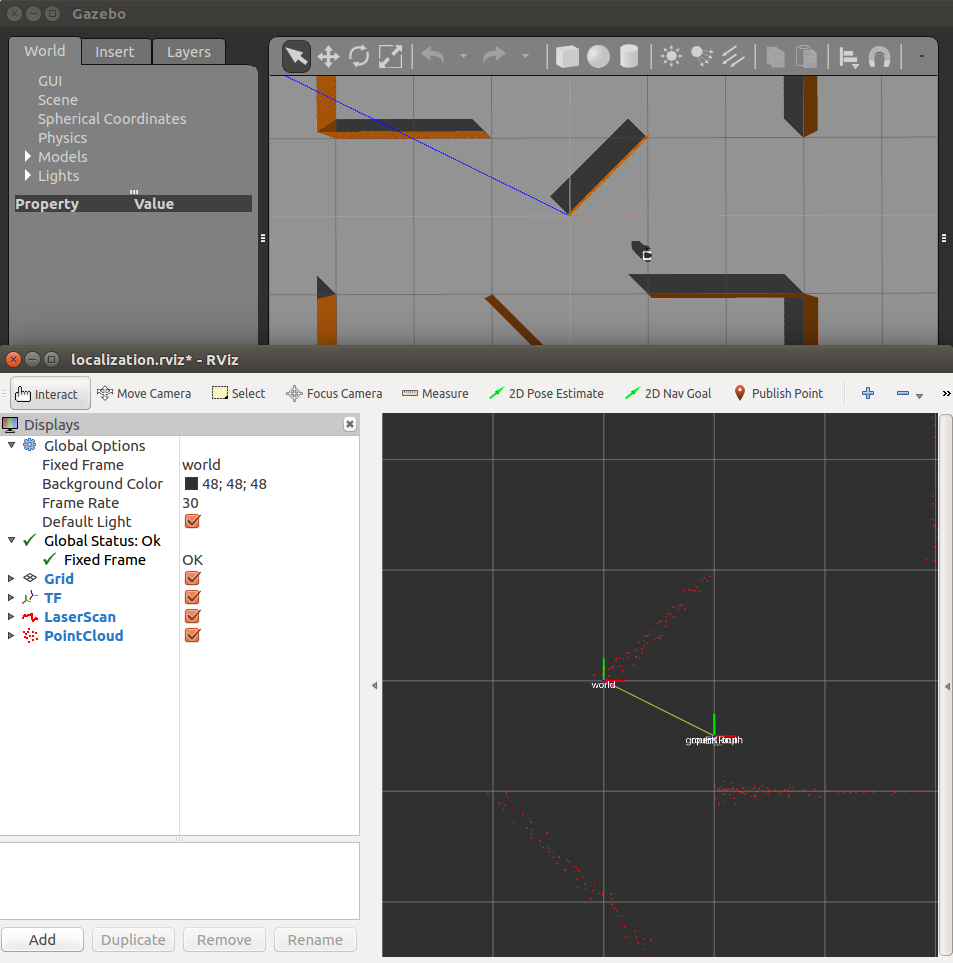
\includegraphics[width=0.9\textwidth]{img/p1-initial.png} \\
	\hline
	Initial state \\
\end{tabular}

\begin{tabular}[t]{l}
	\hline \\
	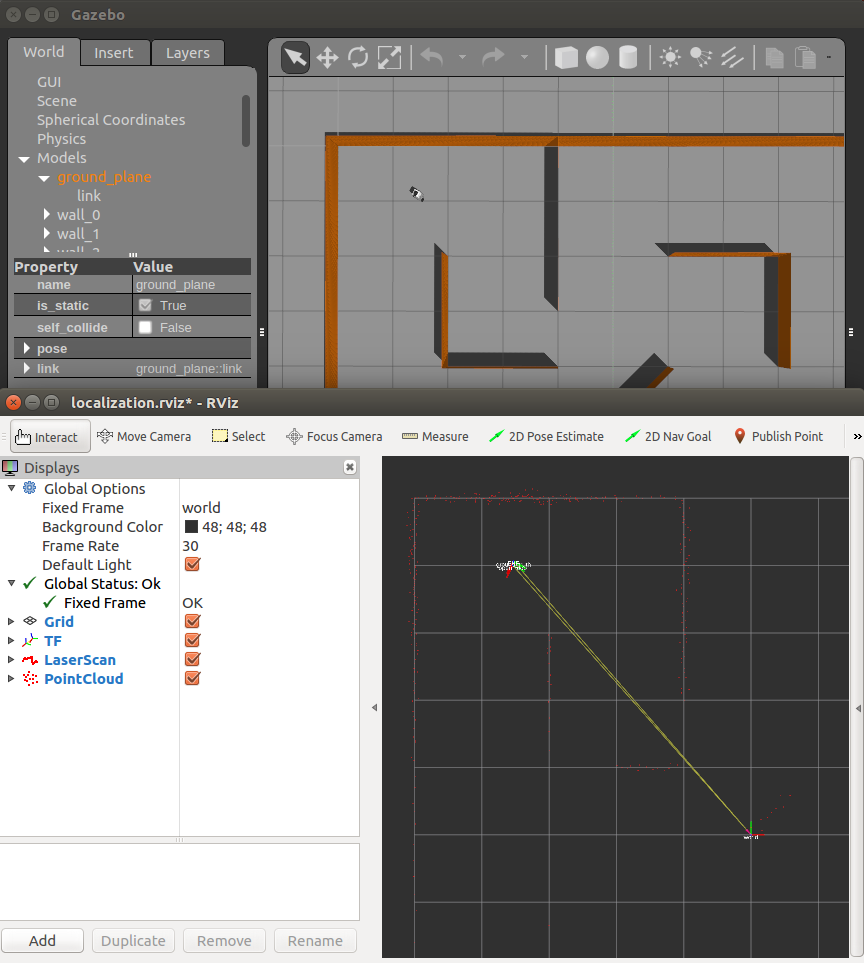
\includegraphics[width=0.9\textwidth]{img/p1-far.png} \\
	\hline
	After moving far \\
\end{tabular}

\begin{tabular}[t]{l}
	\hline \\
	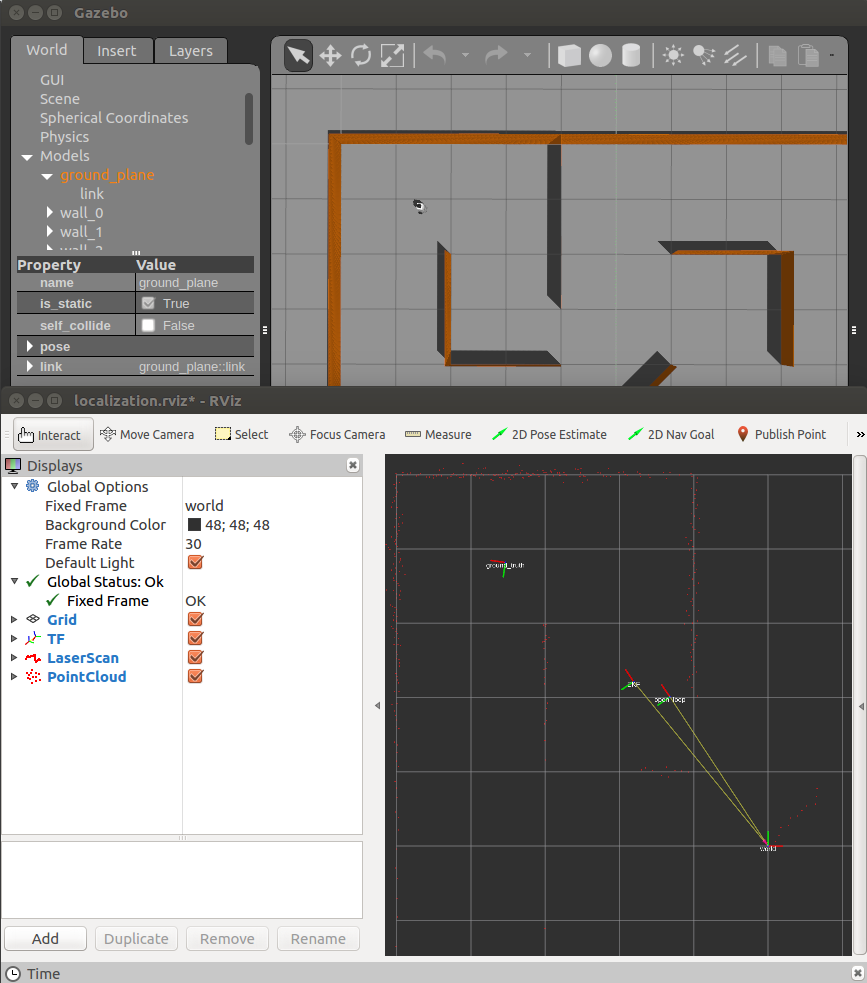
\includegraphics[width=0.9\textwidth]{img/p1-drift.png} \\
	\hline
	State drift \\
\end{tabular}

\end{enumerate}

\section*{Problem 2: EKF SLAM}
\begin{enumerate}[label=(\roman*)]
\item % (i)
(code)

\item % (ii)
(code)

\item % (iii)
It's the same as before; fast movements, abrupt stops, and cumulative errors from having moved a long distance, all contribute to state divergence. As mentioned in the pset, if the robot can only view one wall, then it will be uncertain about its position with respect to the direction parallel to the wall. This is due to state aliasing.

\begin{tabular}[t]{l}
	\hline \\
	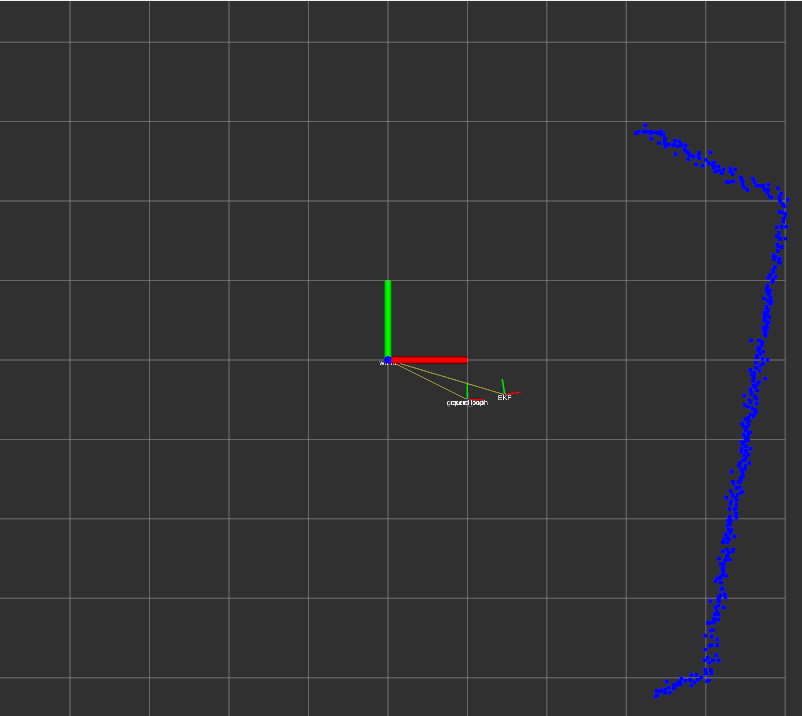
\includegraphics[width=0.9\textwidth]{img/p2-initial.png} \\
	\hline
	Initial state \\
\end{tabular}

\begin{tabular}[t]{l}
	\hline \\
	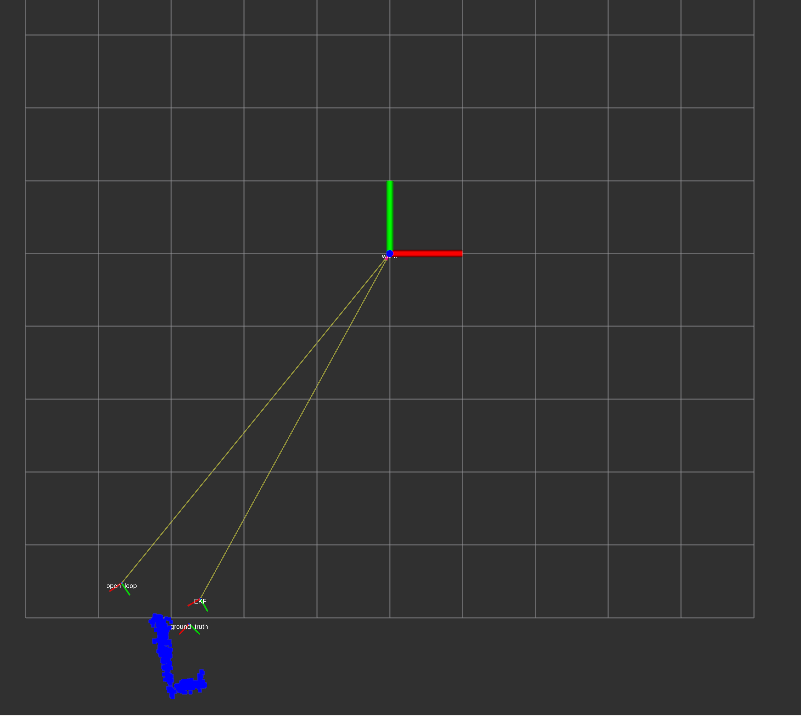
\includegraphics[width=0.9\textwidth]{img/p2-far.png} \\
	\hline
	After moving far \\
\end{tabular}

\begin{tabular}[t]{l}
	\hline \\
	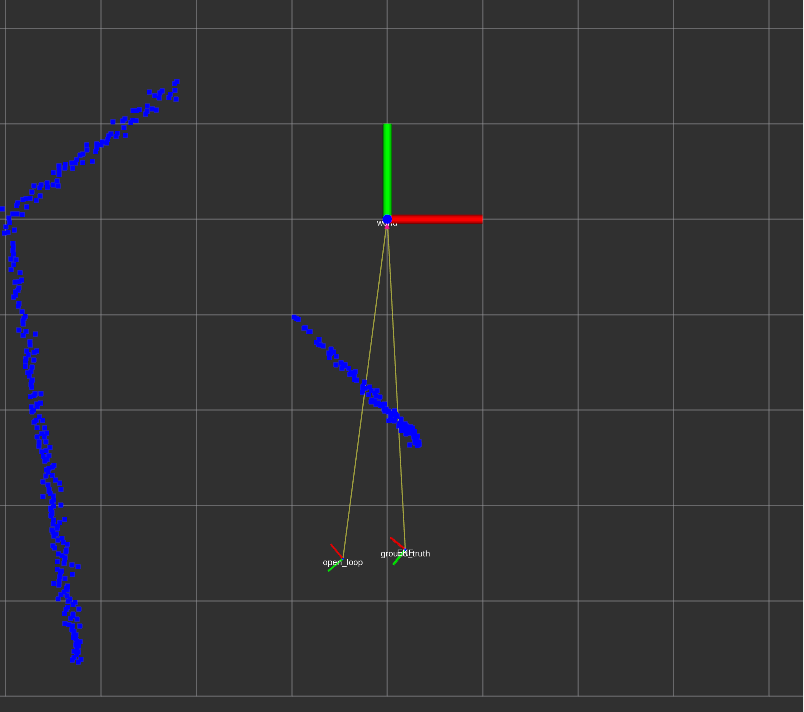
\includegraphics[width=0.9\textwidth]{img/p2-converge.png} \\
	\hline
	Convergence \\
\end{tabular}

\end{enumerate}

\section*{Extra Credit: Monte Carlo Localization}
\begin{enumerate}[label=(\roman*)]
\item % (i)
(code)

\item % (ii)
(code)

\item % (iii)
(code)

\item % (iv)
Causes of divergence are the same as before. However, when running with 1k particles or above, MCL is much more resilient to divergences in state, and the estimated state converges back to ground truth a lot sooner. However, due to the stochastic nature of the algorithm, the state estimate can jitter in place when neither the robot or the world is moving. As expected, convergence is better with more particles by the very nature of Monte Carlo sampling.

\begin{tabular}[t]{l}
	\hline \\
	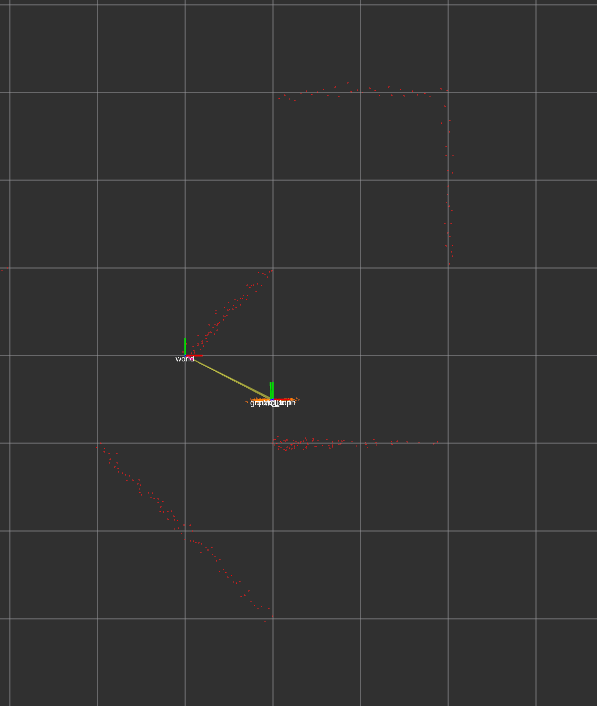
\includegraphics[width=0.9\textwidth]{img/p3-initial.png} \\
	\hline
	Initial state \\
\end{tabular}

\begin{tabular}[t]{l}
	\hline \\
	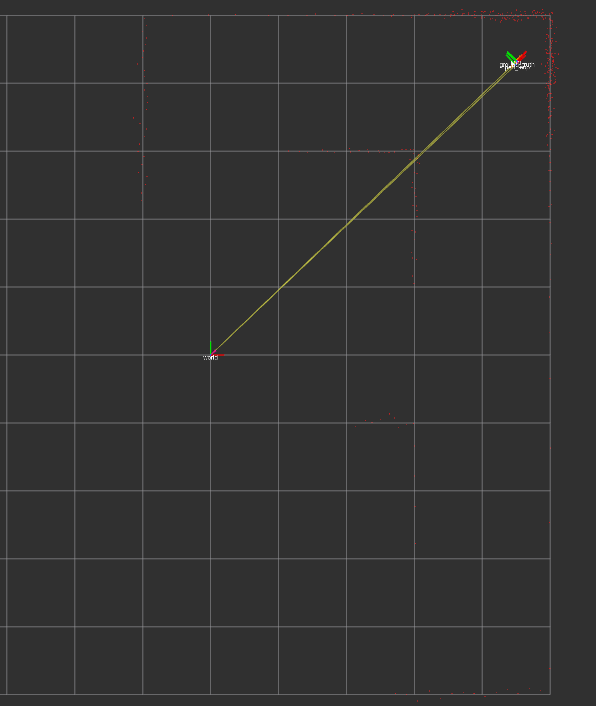
\includegraphics[width=0.9\textwidth]{img/p3-far.png} \\
	\hline
	After moving far \\
\end{tabular}

\begin{tabular}[t]{l}
	\hline \\
	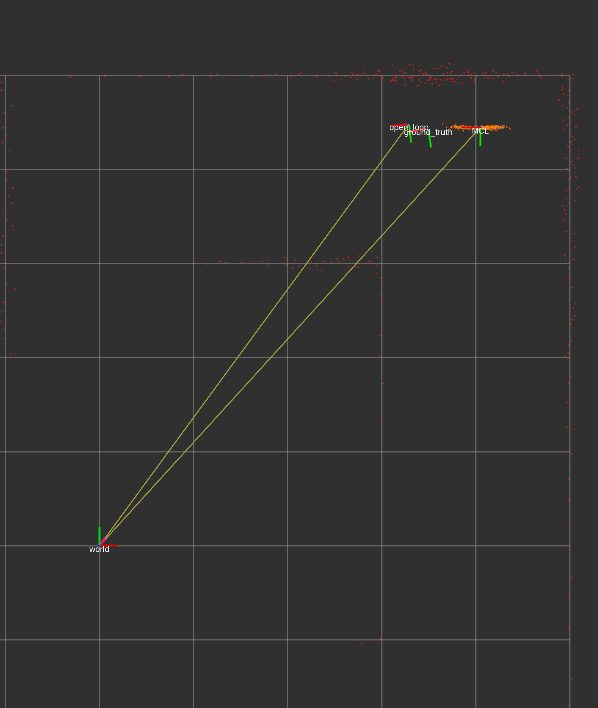
\includegraphics[width=0.9\textwidth]{img/p3-diverge.png} \\
	\hline
	State divergence \\
\end{tabular}

\item % (v)
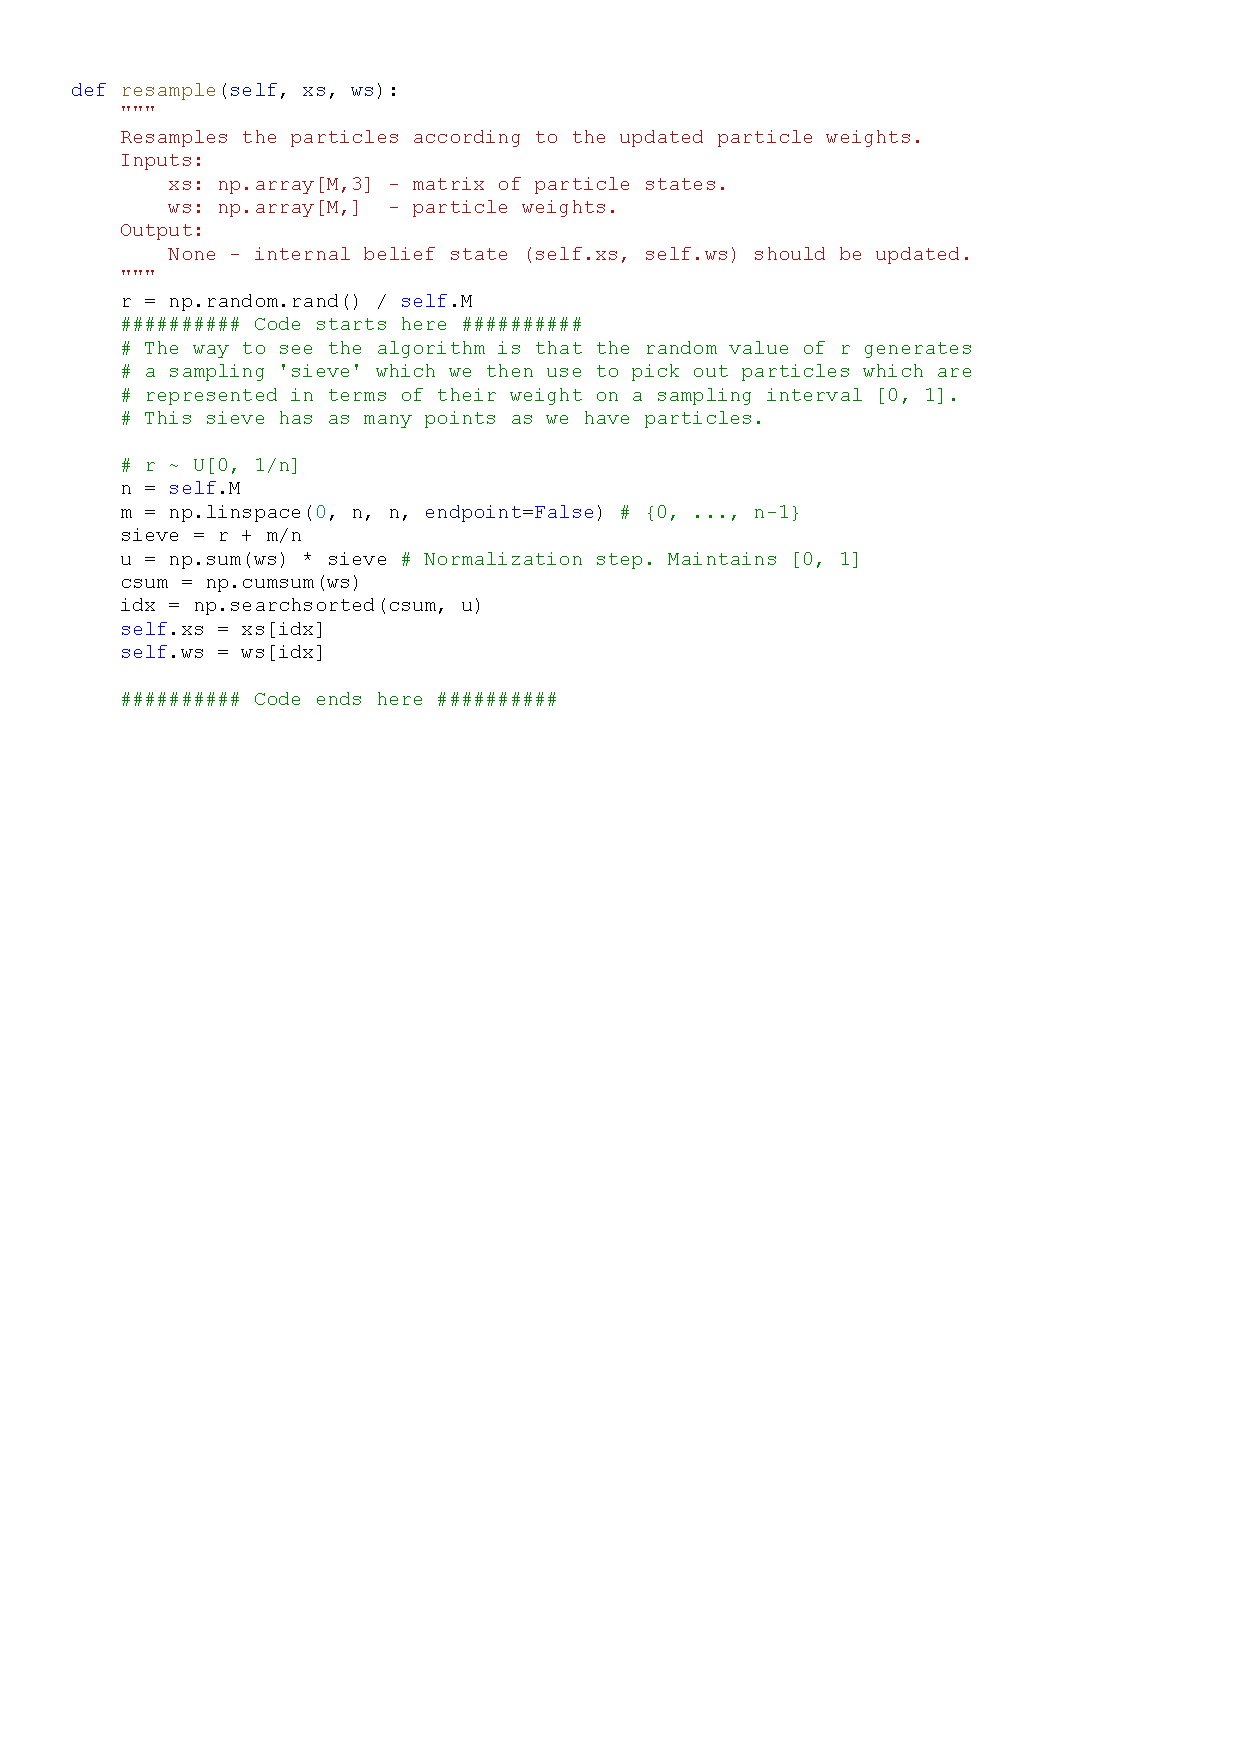
\includepdf[scale=0.9,pagecommand=]{md/resample.pdf}
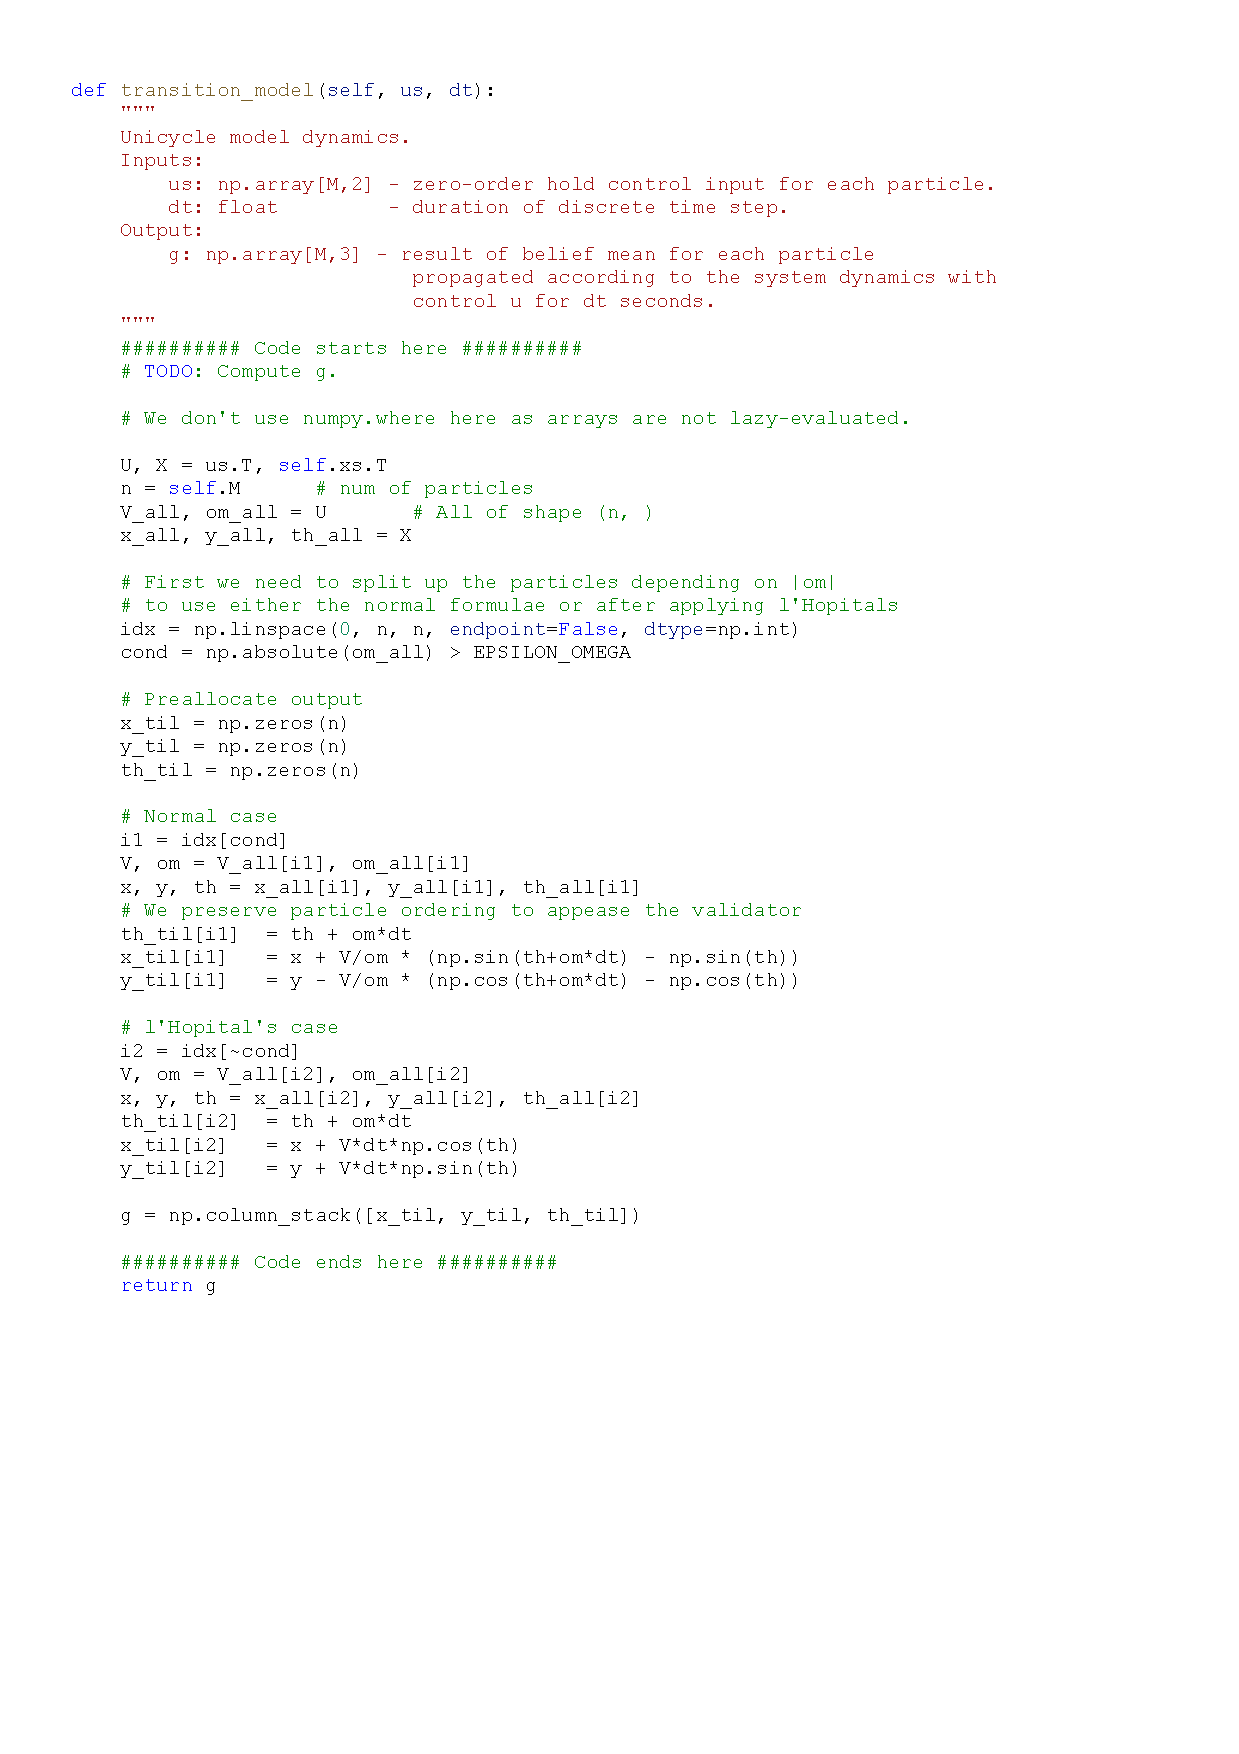
\includepdf[scale=0.9,pagecommand=]{md/transition_model.pdf}
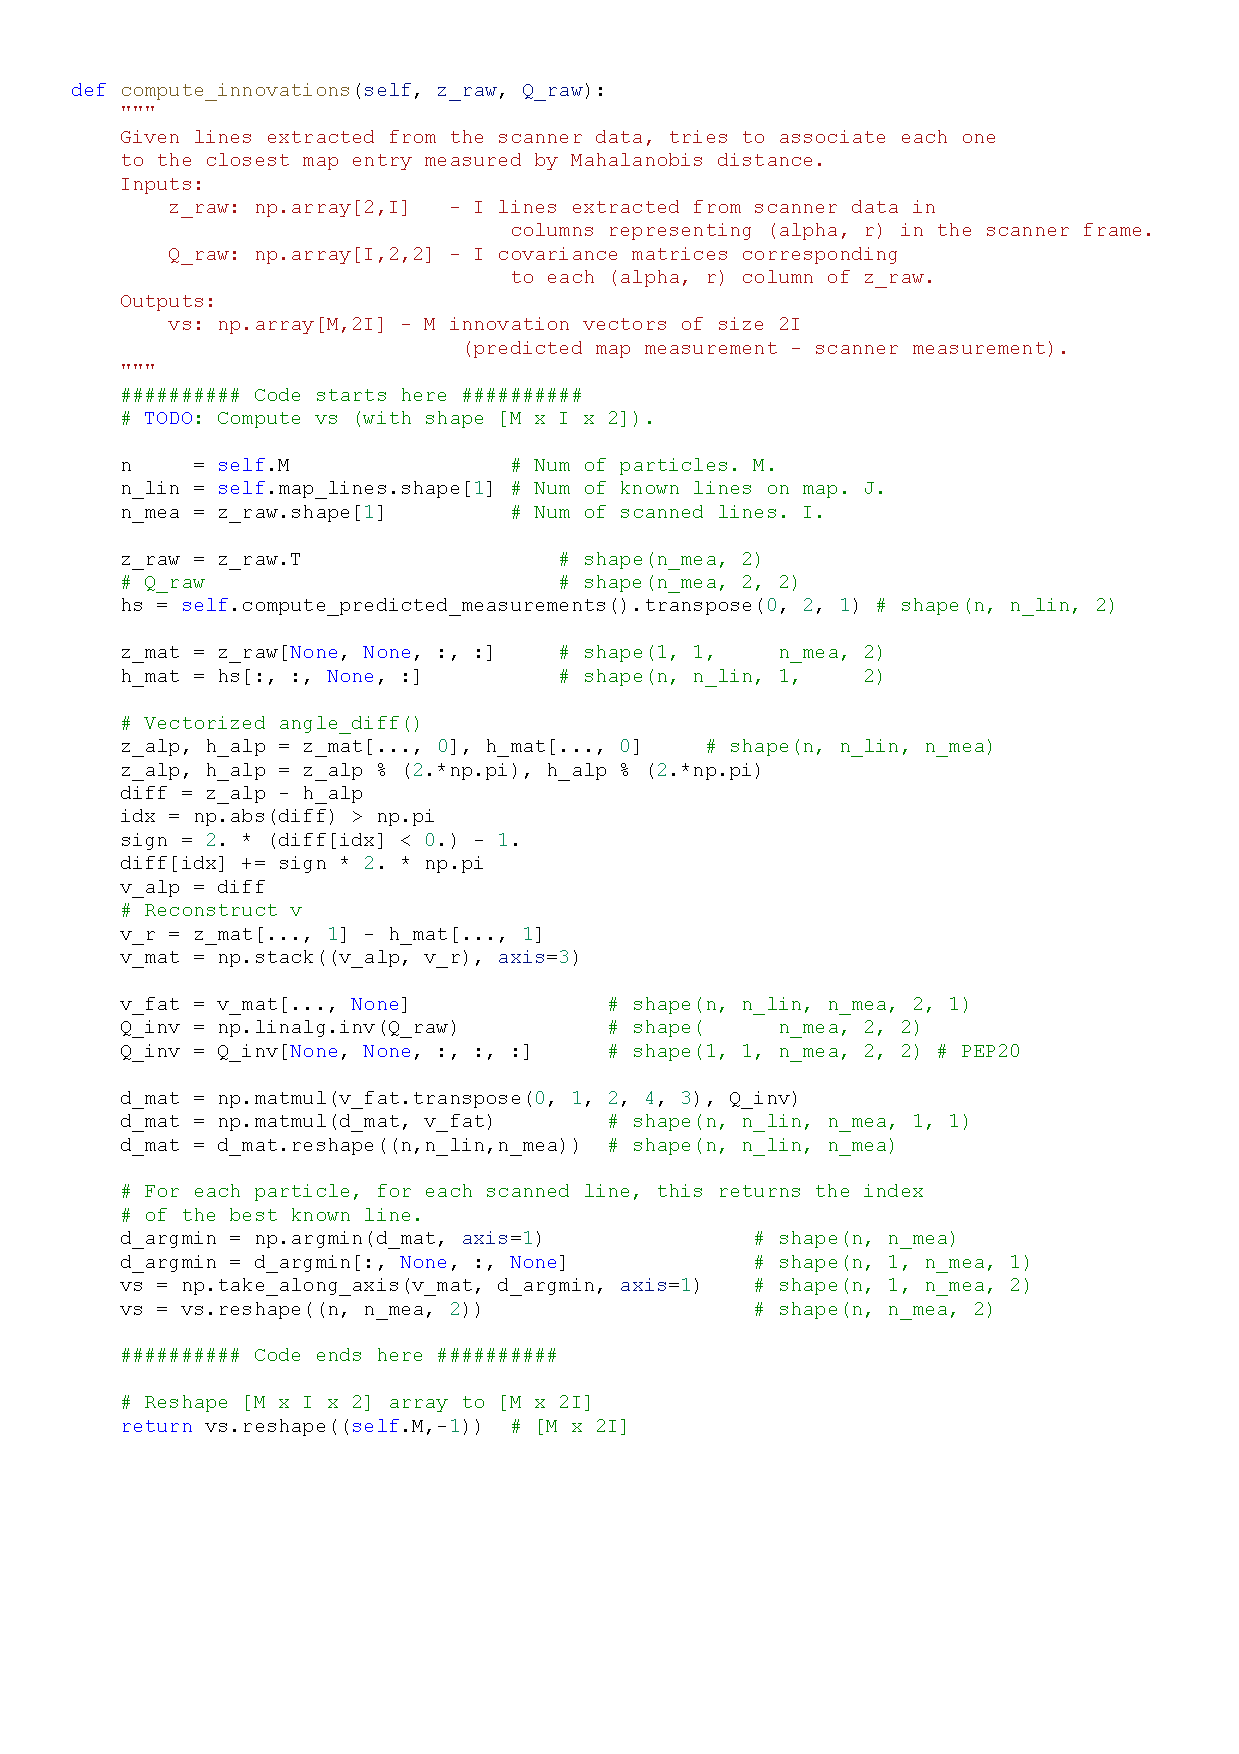
\includepdf[scale=0.9,pagecommand=]{md/compute_innovations.pdf}
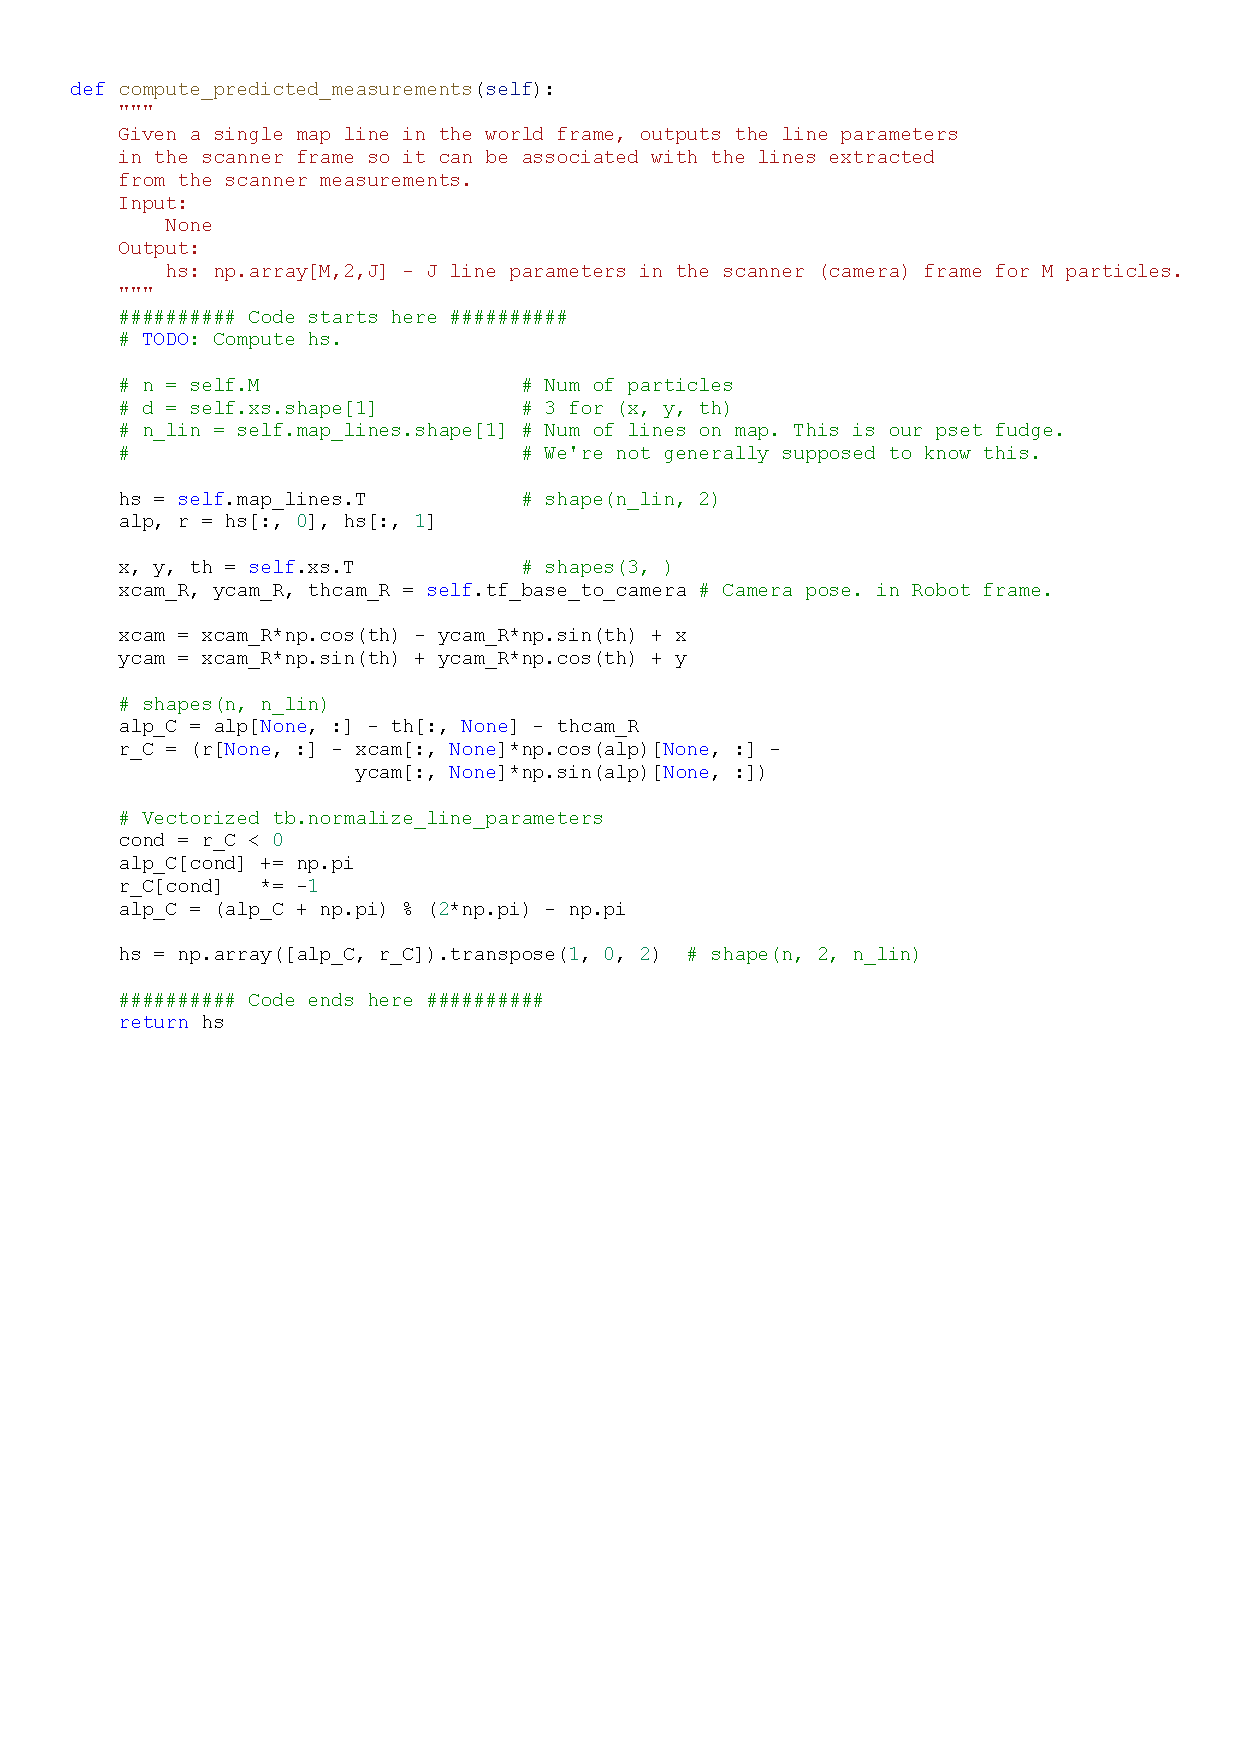
\includepdf[scale=0.9,pagecommand=]{md/compute_predicted_measurements.pdf}

\end{enumerate}

\end{document}
